\documentclass{ximera}

\title{Function Transformations Activity}
\author{MATH 425: Calculus I}

\begin{document}
\begin{abstract}
    Working with the peers in your group, solve the following problems. Make sure to show and justify all your work. Make sure everyone in the group understands the solution and participates. Be prepared to report your answers to the whole class. 
\end{abstract}
\maketitle


In this activity you will learn about the basic transformations we can apply to a function.  This activity is based on a Desmos activity by Dr. David Benson.

\begin{exercise}

Take a moment or two to familiarize yourself with the graph of the absolute value function $y=|x|$. 
\begin{center}
\desmos{ebip7asxmj}{800}{600}
\end{center}

Note that the ``corner'' of the function is at the the origin, the point $(0,0)$.

We will apply these ideas to other functions, but this function makes it easy to see what is going on.
 
Given any real number $c$, there are several ways $c$ can interact with our function $f(x)$.  \begin{enumerate}
    \item $f(x)+c$
    \item $f(x+c)$
    \item $cf(x)$
    \item $f(cx)$
\end{enumerate}

Each of these will transform the graph of $f(x)$ in different ways.  Let's discover how each transformation behaves.  

Before we proceed, notice that the first two transformations involve addition, whereas the latter two transformations involve multiplication.  Also, note that the first and third transformation alter the output and the second and fourth transformations alter the input.  

\begin{enumerate}
    \item Transformation 1: $f(x)+c$.  Use the slider for $c$ on Desmos to investigate transformation 1.  Describe in words what the transformation $f(x)+c$ does to the graph of $f(x)$.  Be specific about what happens with positive and negative values of $c$.
    \begin{center}
      \desmos{3d8w2iohrr}{800}{600}
    \end{center}
    \textcolor{blue}{When $c$ is positive, the graph shifts up by $c$ units.  When $c$ is negative, the graph shifts down by $|c|$ units.}
    \vspace{3in}
    \item Transformation 2: $f(x+c)$.  Use the slider for $c$ on Desmos to investigate transformation 2.  Describe in words what the transformation $f(x+c)$ does to the graph of $f(x)$.  Be specific about what happens with positive and negative values of $c$.
    \begin{center}
      \desmos{qnnzogbjsw}{800}{600}
    \end{center}
    \textcolor{blue}{When $c$ is positive, the graph of $f$ shifts left by $c$ units.  When $c$ is negative, the graph of $f$ shifts $|c|$ units to the right.}
    \vspace{2in}
    \item Transformation 3: $cf(x)$.  Use the slider for $c$ on Desmos to investigate transformation 3.  Describe in words what the transformation $cf(x)$ does to the graph of $f(x)$.  Be specific about what happens with positive and negative values of $c$.
    \begin{center}
      \desmos{49wel3zutx}{800}{600}
    \end{center}
    \textcolor{blue}{When $c$ is positive and greater than 1, the graph gets taller (expands vertically), and when $c$ is positive and less than 1, the graph gets shorter (contracts vertically).  When $c$ is negative, the graph also is reflected over the x-axis}
    \vspace{2in}
    \item Transformation 4: $f(cx)$. Use the slider for $c$ on Desmos (slide 9) to investigate transformation 4.  Describe in words what the transformation $f(cx)$ does to the graph of $f(x)$.  Be specific about what happens with positive and negative values of $c$.\\
    \begin{center}
      \desmos{cruhitjk7c}{800}{600}
    \end{center}
    \textcolor{blue}{When $c$ is positive and greater than 1, the graph of $f$ gets skinnier (contracts horizontally).  When $c$ is positive and less than 1, the graph of $f$ gets wider (expands horizontally).  If $c$ is negative, the graph appears to do the same thing as when $c$ was positive (reflection over an axis of symmetry)}
    \vspace{3in}
    Let's take a closer look at those last two transformations with a different function, $g(x)= \frac{1}{x}+x^3$.  Use the sliders for $n$ on Desmos  to investigate the effects of transformation 3 and 4 on $g(x)$.  
    \begin{center}
      \desmos{lbcucgkkkq}{800}{600}
    \end{center}
    \item What is the difference between $g(cx)$ and $cg(x)$? Think horizontal and vertical.\\
    \textcolor{blue}{hen $c$ is inside the function notation, the function expands or contracts horizontally, and in the opposite way one would think ($\frac1c$ is growth by a factor of $c$ while $c$ is contraction by a factor of $\frac1c$).  When $c$ is outside the function notation, the graph expands or contracts vertically.  }
    \vspace{3in}\\
    Now that we have a baseline to work with, let's explore other functions and think about some terms we'll be using this semester. 
    \item Play with the values of $c$ for each transformation on slide 15 for $f(x)=x^{4}+2x^{3}-13x^{2}-14x+24$.  Pay close attention to the zeroes, hills and valleys. (Click on the circle next to each transformation's equation to turn on the graph.) 
    \begin{center}
      \desmos{6tk3sbszev}{800}{600}
    \end{center}
    \begin{enumerate}
        \item Recall that zeroes of a function (also called "roots" or x-intercepts) are the inputs where the function value is 0.  What are the x-values of the zeroes of the function?\\
        \textcolor{blue}{$x=-4, -2, 1 ,3$}
        \vspace{2in}
        \item What happens to the function's zeroes when $y=2f(x)$?  (Hint: Either think about what you discovered previously, or go back to the previous slide and experiment.)\\
        \textcolor{blue}{The x-values of the zeros stay the same, because this would be a vertical stretch of 2, which leaves what's on the x-axis alone.}
        \vspace{2in}
        \item What happens to the zeroes of the function when $y=f(x)+3$?\\
        \textcolor{blue}{The former zeros are now the x-values of the function for the line $y=3$.  The new zeros are $x=-3.955,-2.1, 1.1, 2.955$}
        \vspace{2in}
        \item What happens to the zeroes of the function when $y=f(2x)$?\\
        \textcolor{blue}{The zeros are half as far from zero, so $x=-2, -1, -0.5, -1.5$}
        \vspace{2in}\\
   Extension: Let's return to our $f(x)$ graph for a minute. 
        \item Where is $f(x)$ increasing?  Where is it decreasing?  (You may need to estimate on some of these points.)\\
        \textcolor{blue}{$f(x)$ is decreasing on $(-\infty, -3.193)$ and $(-0.5, 2.193)$.  $f(x)$ is increasing on $(-3.193, -0.5)$ and $(2.193, \infty)$.}
        \vspace{2in}
        \item What do the "hills" and "valleys" represent?  Do they have a connection with your increasing/decreasing intervals? \\
        \textcolor{blue}{The hills represent maximum values and happen where the function goes from increasing to decreasing.  The valleys represent minimum values and happen where the function goes from decreasing to increasing.}
    \end{enumerate}
\end{enumerate}
    \end{exercise}
    
    \begin{exercise}
    When you complete the function transformations activity, here are a few additional practice problems to work on:
    \begin{enumerate}
        \item If $g(x)=\frac{3x^2+4}{x-2}$, find $g(2)$. Also find and simplify $g(x+h)$.\\
        \textcolor{blue}{$g(2)=\frac{3(2)^2+4}{2-2}$ is undefined because of division by 0. Technically, $x=2$ is not in the domain of $g(x)$ so it doesn't actually make sense to write $g(2)$.\\
        $g(x+h)=\frac{3(x+h)^2+4}{x+h-2}=\frac{3x^2+6xh+3h^2+4}{x+h-2}$}
        \item Sketch a graph of $g(x)=\frac{x-2}{x-3}$.  What is the domain of $g(x)$?  Use your graph to make an educated guess at the range. \\
          \begin{image}
            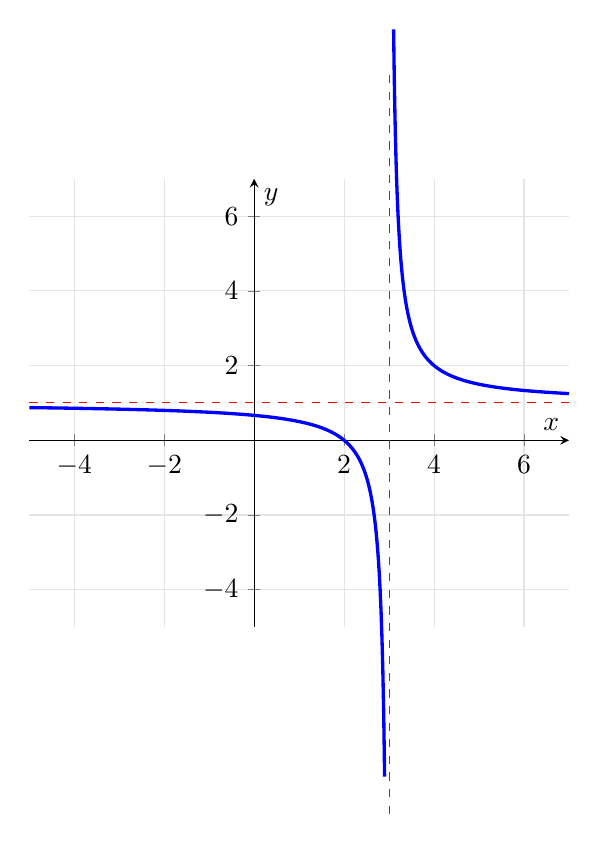
\begin{tikzpicture}
  \begin{axis}[
      axis lines=middle,
      xlabel={$x$}, ylabel={$y$},
      xmin=-5, xmax=7, ymin=-5, ymax=7,
      grid=both, grid style={gray!20},
      clip=false, samples=400
    ]
    \addplot[domain=-5:2.9, very thick, blue, unbounded coords=jump] {(x-2)/(x-3)};
    \addplot[domain=3.1:7,  very thick, blue, unbounded coords=jump] {(x-2)/(x-3)};

    \addplot[dashed, red, samples=2] coordinates {(3,-10) (3,10)}; % x=3
    \addplot[dashed, red, samples=2, domain=-5:7] {1};             % y=1
  \end{axis}
\end{tikzpicture}
          \end{image}
       \textcolor{blue}{ Domain: All real numbers except $x=3$, or $(-\infty,3)\cup(3,\infty)$\\
        Range: All real numbers except for $y=1$ or $(-\infty,1)\cup(1,\infty)$}
        \item The rule $f(x)$ is given by the following table.  Is $f(x)$ a function?  Why or why not?\\
        \begin{tabular}{c|c}
            x & f(x)  \\ \hline
            1 & -4 \\
            2 & -3 \\
            0 & -4 \\
            -1 & 3 \\
            2 & 1
        \end{tabular}
        \textcolor{blue}{$f(x)$ is not a function because there are two outputs associated with $x=2$.}
    \end{enumerate}
\end{exercise}






\end{document}